% Dokumentklassen sættes til memoir.
% Manual: http://ctan.org/tex-archive/macros/latex/contrib/memoir/memman.pdf
\documentclass[a4paper,10pt]{article}
\usepackage[a4paper]{geometry}
% Danske udtryk (fx figur og tabel) samt dansk orddeling og fonte med

% danske tegn. Hvis LaTeX brokker sig over æ, ø og å skal du udskifte
% "utf8" med "latin1" eller "applemac". 
\usepackage[utf8]{inputenc}
\usepackage[danish]{babel}
\usepackage[T1]{fontenc}
 
\usepackage{cite}
\usepackage{natbib}
% Matematisk udtryk, fede symboler, theoremer og fancy ting (fx kædebrøker)
\usepackage{amsmath,amssymb}
\usepackage{bm}
\usepackage{amsthm}
\usepackage{tikz}
%\usepackage{mathtools}
% Kodelisting. Husk at læse manualen hvis du vil lave fancy ting.
% Manual: http://mirror.ctan.org/macros/latex/contrib/listings/listings.pdf
\usepackage{listings}
\usepackage{verbatim}
 
% Fancy ting med enheder og datatabeller. Læs manualen til pakken
% Manual: http://www.ctan.org/tex-archive/macros/latex/contrib/siunitx/siunitx.pdf
%\usepackage{siunitx}
% Indsættelse af grafik.
\usepackage{graphicx}
%\usepackage{bussproofs}

% Reaktionsskemaer. Læs manualen for at se eksempler.
% Manual: http://www.ctan.org/tex-archive/macros/latex/contrib/mhchem/mhchem.pdf
%\usepackage[version=3]{mhchem}
\author{Lau Skorstengaard, 20103173 \\Christian Budde Christensen, 20103616}
\title{Serverbaseret Webprogrammering\\4. Aflevering}

\begin{document}
\maketitle
\section*{Opgave 1}
De mest relevante filer til besvarelsen af denne opgave finde i mappen \texttt{week4/JokeXACT/src/joke}, hvor \texttt{Joke.xact} er xact filen, der laver jokesiden, \texttt{jokes.xml} indeholder de jokes, som der skal præsenteres i xhtml. Slutteligt er \texttt{jokeTemplate.xml} en template, som xact filen bruger. Grunden til, at vi har afleveret mere end blot de fire ovennævnte filer, er, så man let kan analysere med XACT.

Da der ikke var angivet en specifikation for, hvad en jokes XML-fil skal indeholde, så har vi løst fortolket det. Det betyder blandt andet, at attributer er blevet valgfri.

\section*{Opgave 2}
I opgaven bliver man bedt om at bruge analysen fra XACT til at rette et par XACT filer til, så de outputter gyldig XHTML. Vores rettelser resulterer i filerne, der findes i mappen \texttt{Opgave 2}. Det bemærkes, at der ikke var nogle problemer med filen \texttt{Example1.xact}, så den er ikke blevet afleveret.
\subsection*{Exampe 2}
I denne del hører filerne \texttt{Example2.xact} og \texttt{example.xml}. Outputtet fra Xact var:
\begin{lstlisting}
     [java]    Line -1> Result of plug statement is never used.
\end{lstlisting}
Denne fejl fik os til at lede efter et sted, hvor noget bliver sat i et gap, uden det bliver gemt. Dette fandt vi og gemte det i variablen xml.
\begin{lstlisting}
     [java]    Line -1> the gap 'WELCOME' is absent
\end{lstlisting}
For at rette dette kiggede vi i XML templaten og så, at der ikke var et WELCOME gap, men et GREETING gap, så vi rettede WELCOME til GREETING i xact filen.
     [java]    Line -1> maybe plugging XML data into attribute gap 'EMAIL'
Denne del fik os til at gøre flere ting, den første var at fjerne det gap, der er i attributten href og erstatte dette med et kald til getEmail og derefter getString. Derefter flyttede vi den del der gør Emailen bold ned i det XML, som som bliver plugget i GOODBYE gappet, da det ikke må være i attributten.
\begin{lstlisting}
     [java]    Line -1> Problem in {http://www.w3.org/1999/xhtml}body 
     [java]             created at example.xml:5:8 invalid child a
\end{lstlisting}
Tilføjede et namespace præfiksset h til a i det XML, der bliver sat i gappet GOODBYE.
\begin{lstlisting}
     [java]    Line -1> Problem in {http://www.w3.org/1999/xhtml}ul 
     [java]             created at example.xml:8:7 invalid child
     [java]             {http://www.w3.org/1999/xhtml}ul
     [java]    Line -1> Problem in {http://www.w3.org/1999/xhtml}ul 
     [java]             created at example.xml:14:7 invalid child 
     [java]             {http://www.w3.org/1999/xhtml}ul
\end{lstlisting}
Ændrede i addExtraListItems metoden, så den ikke laver et tag der afslutter ul, men i stedet pakker det, man vil indsætte ind i et li elemet og sætter det ind efter alle ul tags.

\subsection*{Example 3}
\begin{lstlisting}
     [java]    Line -1> Problem in {http://www.w3.org/1999/xhtml}a
     [java]             created at example.Example3.makeTableEntry:?:50 
     [java]             invalid child blink
\end{lstlisting}
Blink er \emph{desværre} deprecated, så for stadig at have en eller anden form for fremhævning har vi erstattet det med et bold tag.
\begin{lstlisting}
     [java]    Line -1> Problem in {http://www.w3.org/1999/xhtml}title 
     [java]             created at example3.xml:3:10 invalid child 
     [java]             {http://www.w3.org/1999/xhtml}h1
\end{lstlisting}
Fjernede h1 tagget fra det sted i \texttt{Example3.xact} bliver plugget, da det ikke er lovligt at have i title elementet. Indsatte det i stedet i example3.xml der hvor der er et title element i body.
\begin{lstlisting}
     [java]    Line -1> Problem in {http://www.w3.org/1999/xhtml}img 
     {java]             created at example.Example3.makePicture:?:201
     [java]             required attribute missing alt
\end{lstlisting}
Tilføjede alt tag til img elementet.
\begin{lstlisting}
     [java]    Line -1> Problem in {http://www.w3.org/1999/xhtml}a 
     [java]             created at example.Example3.makePicture:?:50
     [java]             invalid child {http://www.w3.org/1999/xhtml}h3
\end{lstlisting}
Ændrede rækkefølgen af de to tags (dette er fra makePicture metoden).
\begin{lstlisting}
     [java]    Line -1> Problem in {http://www.w3.org/1999/xhtml}p 
     [java]             created at example3.xml:9:16 invalid child 
     [java]             {http://www.w3.org/1999/xhtml}h3
\end{lstlisting}
Fjernede p tag i \texttt{example3.xml}.
\begin{lstlisting}
     [java] example.Example3.makePicture
     [java]    Line -1> the gap 'URL' is absent
\end{lstlisting}
Vi fjerende det UML gap der var forsøgt lavet i attributten og indsatte en reference til lokalvariablen name.
\begin{lstlisting}
     [java]    Line -1> Problem in {http://www.w3.org/1999/xhtml}a 
     [java]             created at example.Example3.makeTableEntry:?:50
     [java]             invalid attribute value href="#&#x0;"
\end{lstlisting}
Fjernede forsøg på at lave gap og erstattede det med en reference til en lokal variabel, link.
\begin{lstlisting}
     [java]    Line -1> Problem in {http://www.w3.org/1999/xhtml}a 
     [java]             created at example.Example3.makePicture:?:63
     [java]             invalid attribute value name=""
\end{lstlisting}
Fjernede a tag og gav elementet h3 en attribut id, som kan refereres fra det andet link tag.
\begin{lstlisting}
     [java]    Line -1> Problem in {http://www.w3.org/1999/xhtml}a 
     [java]             created at example.Example3.makeTableEntry:?:50
     [java]             invalid attribute value href="#&#x0;"
     [java]    Line -1> Problem in {http://www.w3.org/1999/xhtml}div 
     [java]             created at example.Example3.makePicture:?:52
     [java]             invalid attribute value id="0"
\end{lstlisting}
Dette løste vi ved at fjerne den statiske variabel og lave en lokal variabel i main, som holder styr på et id. Dette id bliver givet som argument til de metoder, der bruger det. I de to metoder bliver der givet et præfiks til det tal der er kommet med som argument, hvilket bliver gemt i en lokalvariabel og refereret fra den attribut, der skal bruge det.

Dette er umiddelbart for meget arbejde, hvor noget af det skyldes, en mangel på forståelse af hvad problemet var (skulle vi gør det nu ville vi nok blot give id'et et præfiks direkte).\\\\
Dette afslutter hvad vi har gjort for at rette fejlene. XACTs analyse er blevet brugt til at pege os i den rigtige retning, dog har de også været lidt forvirrende, da vi på et tidspunkt sad med:
\begin{lstlisting}
     [java]    Line -1> maybe plugging XML data into attribute
     [java]             gap '0GENERATEDGAP0'
\end{lstlisting} 
Hvilket tydelig vist er et autogenereret gap, men vi vidste ikke, hvorfor det ikke blev fyldt ud. Vi fandt senere ud, at det var fordi, vi gav et XML objekt videre til en attribut, der skulle udfyldes, men den forventer en String.
\section*{Opgave 3}
Den originale \texttt{GuessingGame.xact} gemte og beregnede XHTML i \texttt{UserState} objektet. Denne ville også indeholde alle \texttt{SubmitHandler} objekter, som direkte ændrede i XHTML outputtet og sendte det til klienten ved hjælp af \texttt{update} metoden. Spillet havde kun tre metoder \texttt{start}, \texttt{play} og \texttt{record}. \texttt{start} sørgede for at starte spillet og initalisere brugerens ``session'', \texttt{record} viste hvem, der havde hiscoren og \texttt{play} stod for at vise spillet. Som sagt havde session-objektet al ansvar for at vise spillet. Hver gang en form blev submitted, ville handleren enten tilføje en besked til en form-template eller rydde indholdet og tilføje noget nyt. Dette afspejlede ikke control-flowet særlig godt og førte hurtigt til flere nested if's. 
\section*{Opgave 4}
\begin{center}
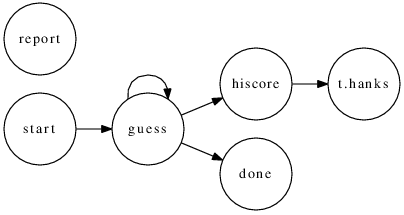
\includegraphics[width=10cm]{graphs/g0.png}
\end{center}
Controlflowet er afbilledet i ovenstående graf. Ud fra denne har vi lavet metoderne \texttt{guess},  \texttt{done},  \texttt{hiscore} og  \texttt{thanks}. Der navigeres mellem disse metoder via submit handlers, som returnerer en URL afhængig af brugerens handlinger. Der er dessuden tilføjet et filter, som sørger for at ingen ufortjent sætter sig selv på highscoren.  
\section*{Opgave 5}
Den største forskel mellem JWIG og Struts/JSF er fokus på XML's korrekthed, dette medfører flere garantier for sidens korrekthed, og dermed større modstandskraft mod eksempelvis XSS angreb. Derudover kræver frameworket minimal konfiguration og kedelige, trivielle opgaver, som form submit er abstraheret væk for udvikleren. JWIG har både komponenter af action-baserede framworks, som Struts, og component-baserede frameworks, som JSF.  

 
\end{document}

